	
	This thesis investigates methods for gaining customer insights using graph
	machine learning. Graph machine learning is a current frontier in machine 
	learning and has many successful applications in many areas such as recently 
	shown by the success of AlphaFold \citep{senior2020improved}. AlphaFold made 
	a breakthrough for predicting protein structures where they made use of the 
	observation that a folded protein can be considered as a spatial graph 
	\citep{AlphaFoldTeam2020}. More generally, there are a vast range of 
	applications for graph machine learning in the fields of natural science, 
	social science and many more as shown by the excellent overview given by 
	\cite{zhou2020graph}. Graphs are especially useful as they allow for the 
	consideration of relationships between observations. Graph machine learning 
	has for that reason become a promising field as it allows for the use of
	richer data. This thesis will focus on graph machine learning for the
	purpose of customer classification. In particular, it is investigated to
	what extent semi-synthetic graphs can be used for graph machine learning.
	To provide a better overview as to how this topic relates to business \& 
	economics related fields such as gaining customer insights, some motivating
	examples are provided in the following section. 
	
	\section{Relevance to Economics}

	\noindent From a business \& economics perspective, graphs are particularly
	interesting if one wants model the interactions between institutions. An 
	example for this is shown in an article published by 
	\cite{schweitzer2009economic} which created a graph showing the 
	interdependencies of international banks as a network shown in figure 
	\ref{fig:bank_network}. Graphs can be useful tool for illustrating such 
	interdependencies and provides important information for making the banking 
	system more robust and resilient. 

	\begin{figure}[h]
		\centering
		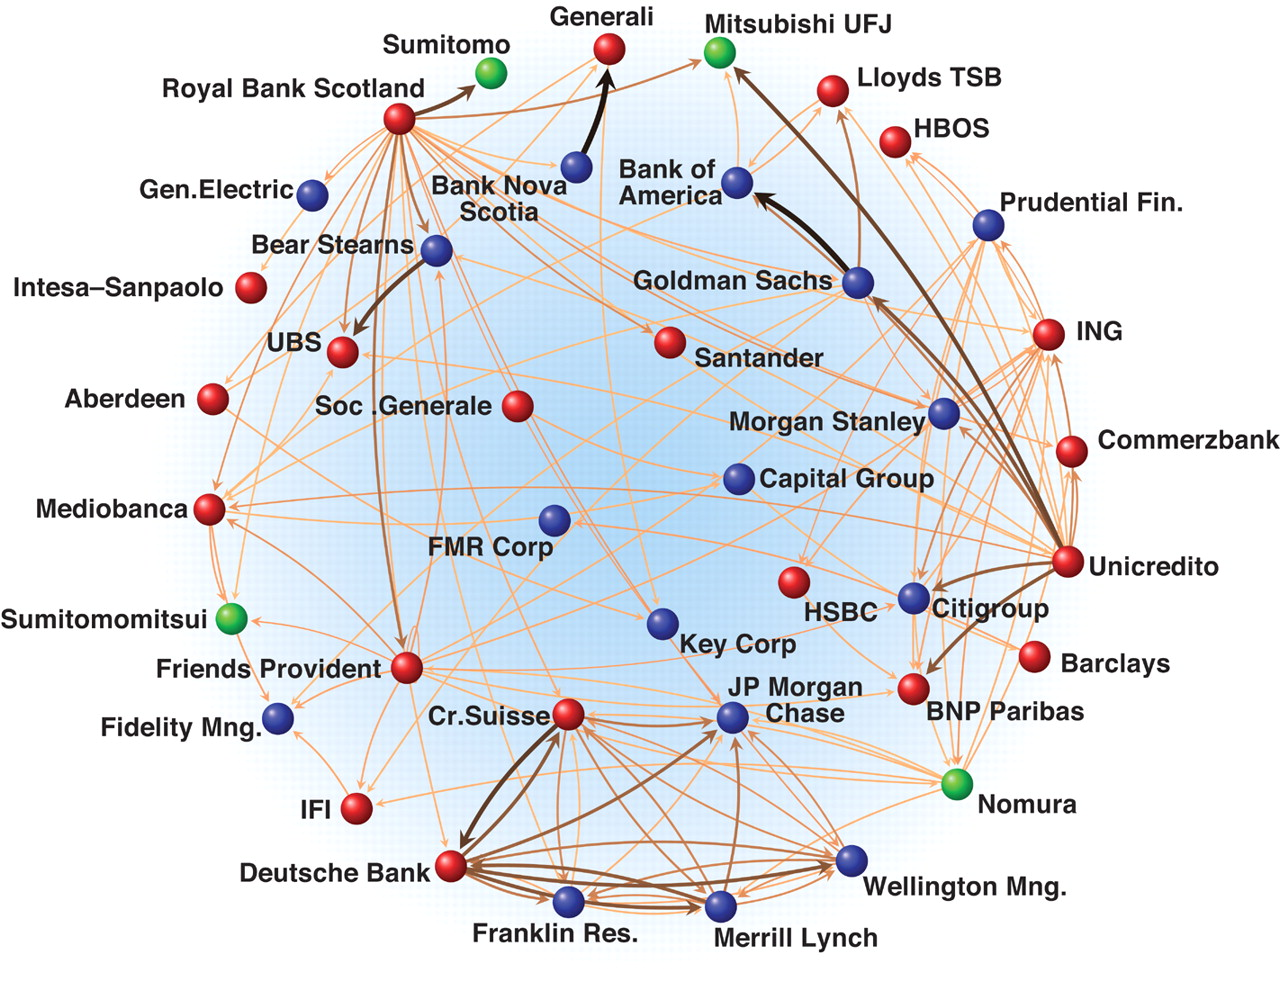
\includegraphics[width=0.5\textwidth]{bank_network.jpg}
		\caption{Bank Network}
		\cite[p. 424]{schweitzer2009economic}
		\label{fig:bank_network}
	\end{figure} 

	\noindent Another interesting application of graphs for business \& 
	economics are social interactions. While there are many different
	interesting applications where social interactions are of interest,
	the focus of this thesis is placed on gaining customer insights for 
	purposes such as improving products \& services as well as marketing. Indeed, 
	this is one of the main areas where social network companies such as 
	Facebook or search providers like Google make their revenue by providing 
	customer insights or selling targeted advertising 
	\citep{Facebook2021,Alphabet2021}. Both Facebook and Google have the 
	advantage, that their businesses naturally capture relational or more 
	generally network data which can be represented as graphs. Most researchers 
	or companies however do not have access to such data. Companies for instance 
	may have access to large amounts of customer data, they however typically 
	would not have access to relational information (e.g. which client is 
	connected with which other clients). The same is true for researchers, where 
	social scientists often collect data via anonymous surveys which makes the 
	collection of network data basically impossible. In most cases this 
	constrains companies or researchers to cross-sectional data with no network 
	information. It is important to mention, that there is a lot of network 
	data available online. This network data however typically only contains the 
	network connections. The important feature data such as demographic data, 
	topic specific variables or labels are however typically not available. 
	Without any feature data, graphs provide rather limited information as they 
	are lacking features and can thus only provide limited information for 
	gaining customer insights. This is an issue in terms of data access and is 
	a frustrating reality which also affects this master's thesis. It however 
	motivates the research topic of this thesis which is presented in section
	\ref{section:research_topics}. First, a general overview of machine
	learning is given in the following section.
	
	\section{Overview Machine Learning}

	This section provides a high-level overview of machine learning and
	will specify the type of machine learning task used in this thesis. To
	start, it is important to correctly categorize machine learning. There are
	many related big topics such as data science, big data or artificial
	intelligence and it is often not clear what exactly is meant. An overview
	of how these different terms can be categorized is shown in figure 
	\ref{fig:ml_overview}.

	\begin{figure}[h]
		\centering
		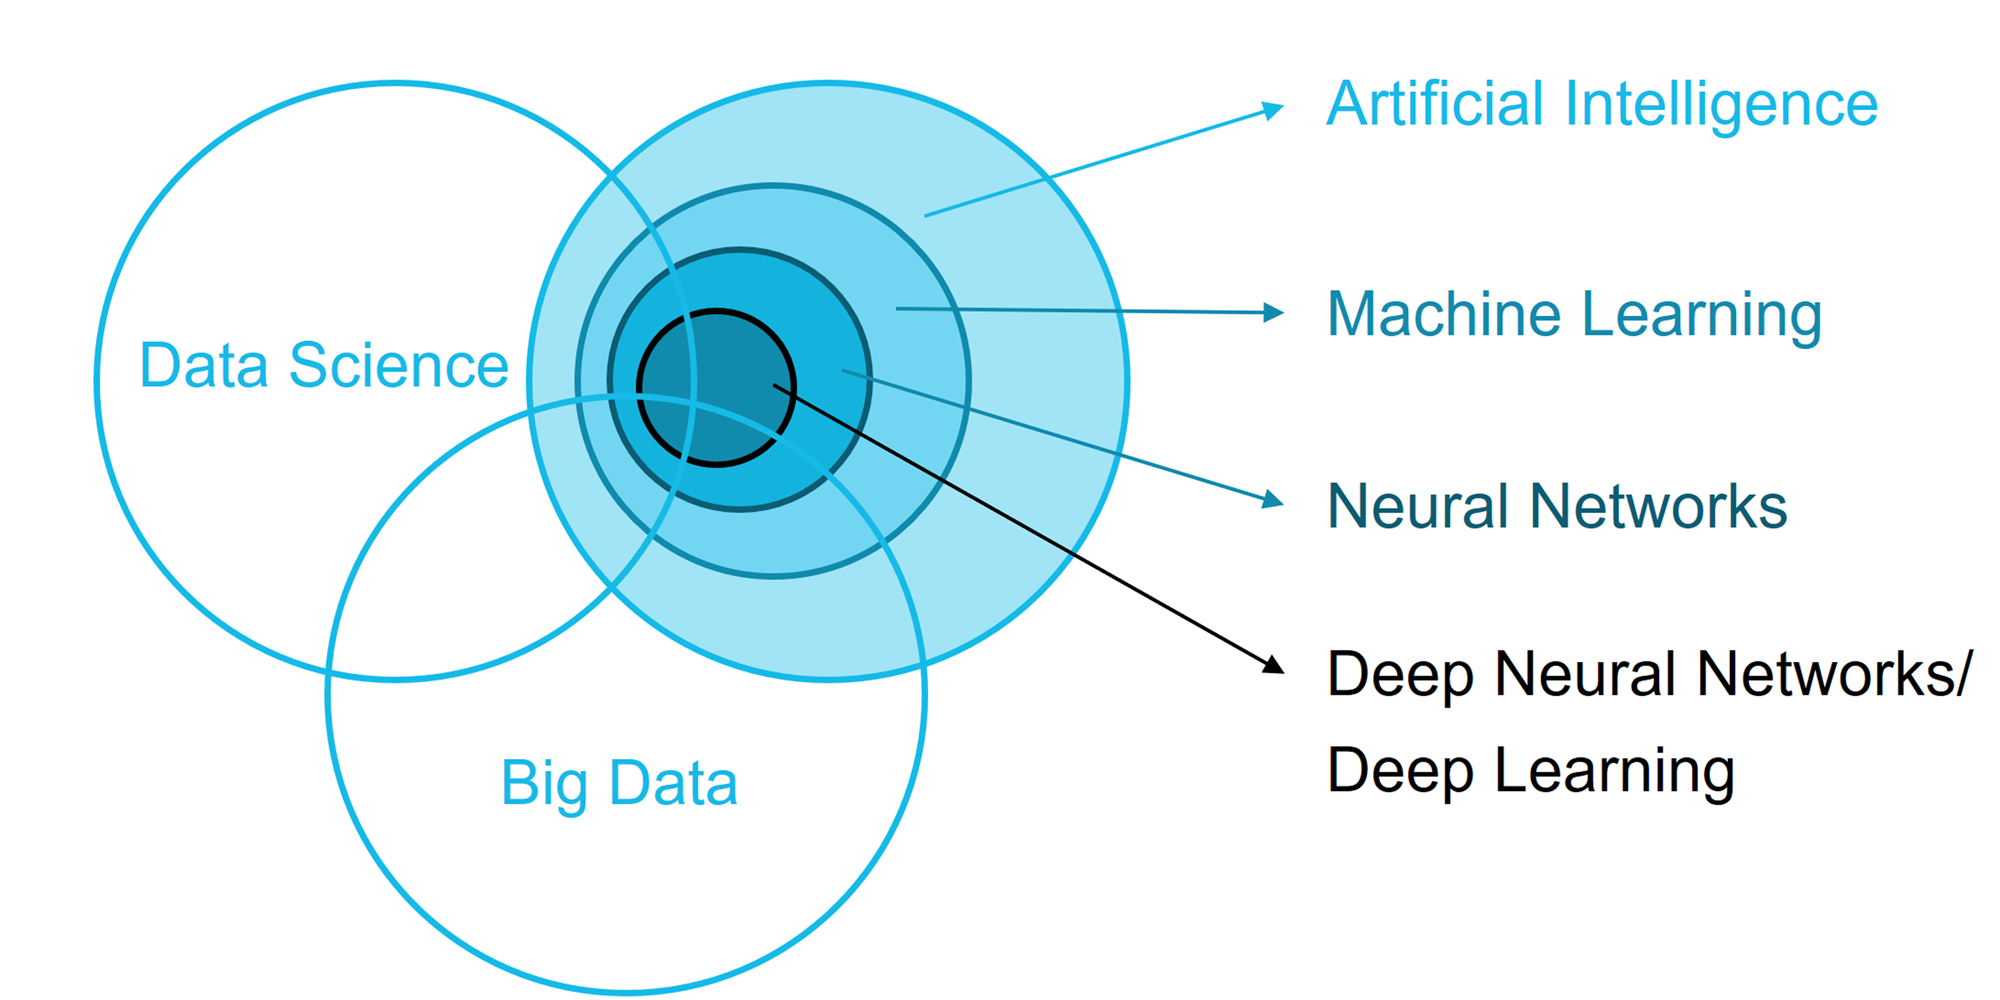
\includegraphics[width=0.7\textwidth]{overview_datascience.png}
		\caption{Overview Machine Learning}
		\citep{Frauenhofer2021}
		\label{fig:ml_overview}
	\end{figure} 

	\noindent Figure \ref{fig:ml_overview} shows well, how these different
	terms are related with each other. Machine learning in particular is
	mostly ascribed to the domain of artificial intelligence. It however also 
	has a shared domain with data science and big data. It is thus at the
	intersection of these three interrelated fields. Machine learning models 
	such as neural networks and deep neural networks are specific models within
	machine learning and are often referred to separately due to their
	popularity. In this thesis, differentiating between machine learning and
	neural networks is not necessary as the considered machine learning models
	will be used for the same task. Machine learning can be applied for various
	tasks and is again best presented visually as shown in figure 
	\ref{fig:ml_tasks}.

	\begin{figure}[h]
		\centering
		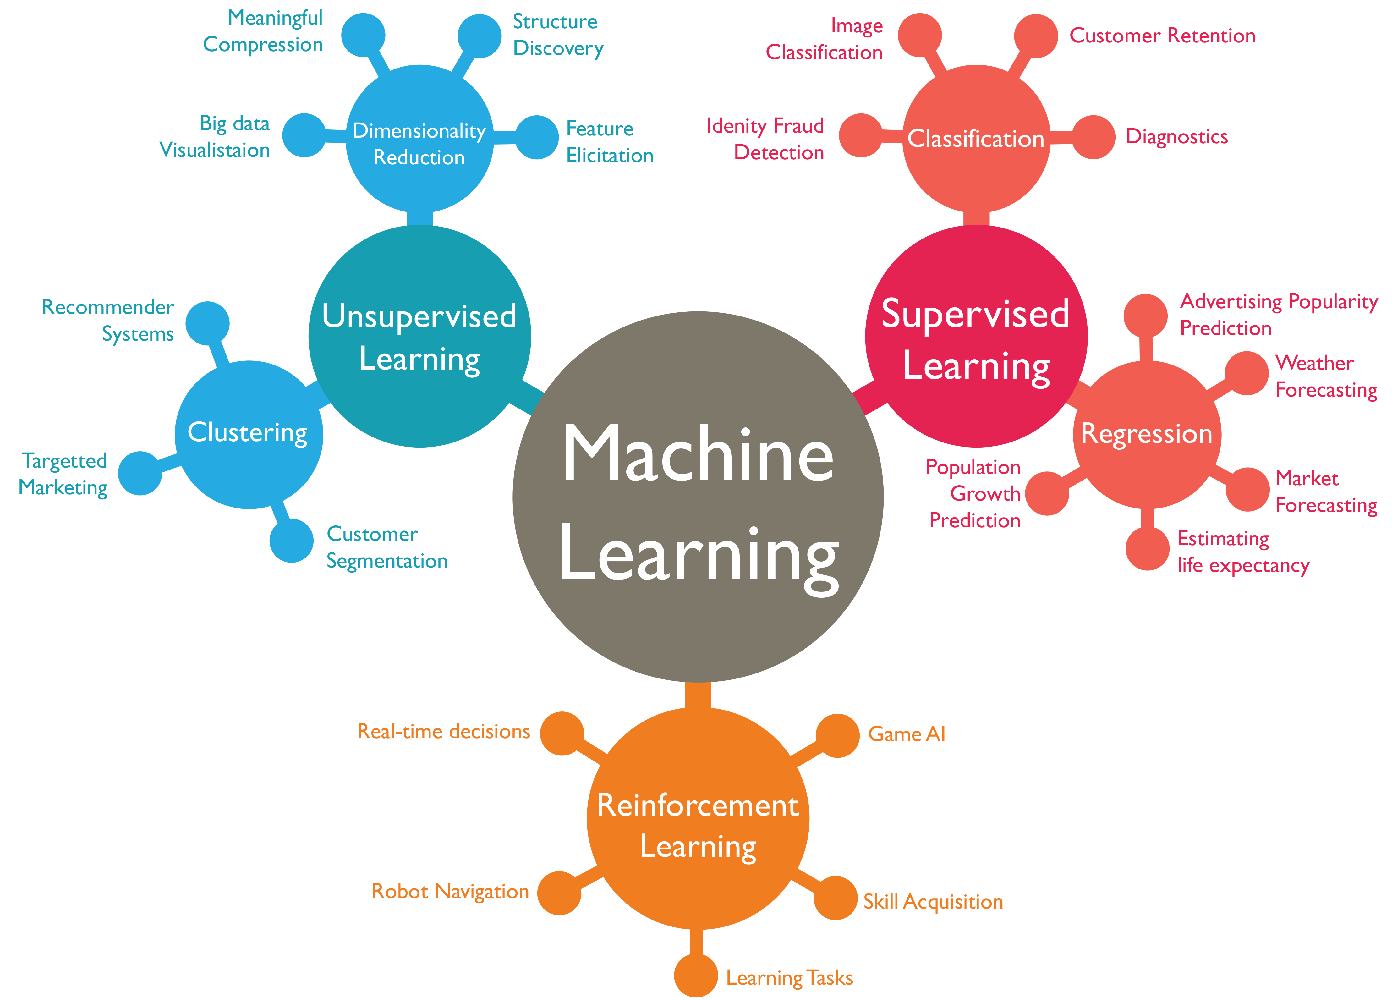
\includegraphics[width=0.8\textwidth]{ml_tasks.png}
		\caption{Overview Machine Learning Tasks}
		\citep{Artisan2020}
		\label{fig:ml_tasks}
	\end{figure} 

	\noindent It is shown in figure \ref{fig:ml_tasks} that the main tasks for
	machine learning involve classification, regression, reinforcement
	learning, clustering and dimensionality reduction. This thesis will focus
	on classification tasks. This task was chosen given the available data and 
	because it allows for a nice comparison of different models. Well known 
	standard machine learning models used for classification tasks include 
	logistic regression \citep{cramer2002origins}, naive bayes 
	\citep{zhang2004bayes}, support vector machines 
	\citep{platt1999probabilistic}, random forest classifiers
	\citep{breiman2001random}, AdaBoost \citep{freund1997decision} and
	artificial neural networks \citep{mcculloch1943logical}. This is an
	incomplete list of popular machine learning models that can be used for
	classification tasks. Classification tasks can be applied for various
	settings such as predicting whether a customer is satisfied or whether to
	grant a mortgage to a client among many others. The aforementioned machine
	learning methods have in common, that they all only consider feature data
	and cannot consider network information. \\

	\noindent Graph machine learning methods are different in that they consider 
	both feature data as well as network information. If one wants to categorize 
	graph machine learning within the framework shown in figure 
	\ref{fig:ml_overview}, it is probably best categorized as a special form of 
	a neural network. It is however not necessarily a deep neural network, as 
	network depth does not necessarily improve the model and can be even 
	counter-productive. Within graph machine learning, there are two main
	approaches. The first approach focuses on learning vector representations
	of graphs which are used for downstream machine learning. The downstream
	machine learning models include the standard models presented previously. 
	Graph representation learning approaches include models such as DeepWalk 
	\citep{perozzi2014deepwalk} and Node2Vec \citep{grover2016node2vec} among 
	others. The second approach involves the application of graph neural 
	networks for which there exist many different approaches. These approaches 
	include models such as Graph Convolutional Networks \citep{kipf2016semi}, 
	GraphSage \citep{hamilton2017inductive} and many more. \\

	\noindent The detailed theoretical background for the considered graph
	machine learning models will be provided in chapter 2.

	\section{Research Topic}
	\label{section:research_topics}

	\noindent The difficult access to graphs which include features, motivated 
	the search for alternatives. A review of the literature revealed, that a 
	form of synthetic graph generation could provide a solution to the data 
	access problem. Classic graph generation procedures include the famous 
	Erdös-Rényi graphs \citeyearpar{erdos1959random}, the small-world model by 
	\cite{watts1998collective}, the well-known model by 
	\cite{barabasi1999emergence} and more recently Kronecker Graphs by
	\cite{leskovec2010kronecker}. These models are all very instructive
	regarding the graph generation process and for understanding graph
	properties. These networks however all have the short-coming, that they do 
	not allow for the assignment of feature data to the nodes/observations in the
	network. It became clear, that one has to find or develop a model which 
	makes use of existing feature data for the graph generation process. 
	\cite{kim2012multiplicative} developed the Multiplicative Attribute 
	Graph (MAG) model. This model makes use of randomly generated feature data 
	which is referred to as attribute data by the authors. The model is shown
	to be capable of generating random graphs which can adhere to observed real 
	world network properties. An analysis of the MAG model reveals, that it 
	could also be a useful model for creating semi-synthetic graphs using 
	existing feature data. For that reason, the MAG model is selected for 
	generating semi-synthetic graphs. This model will be introduced in detail 
	in section \ref{section:theory_graphgen}. \\

	\noindent More recently, researchers have focused their attention to
	generative graph models. These models create graphs with features using
	real graphs as a training input. Examples for such models are Graph
	Recurrent Neural Networks \citep{you2018graphrnn} and deep generative graph
	models \citep{li2018learning}. These are very fascinating models which can
	be used to recreate or scale graph data. For the purpose of this thesis,
	these methods were not purposeful, as it requires an existing graph with
	features to be available. Such a graph is unfortunately not available for
	this thesis. Nevertheless, this is an interesting current topic for graph 
	generation which was considered. \\ 

	\noindent The access problem to graphs including feature data might be resolved
	using the MAG model as previously mentioned. This model is interesting as 
	most researchers or companies have access to large amounts of feature data 
	such as customer databases or feature data which can be created using 
	well-known methods like surveys. For that reason it would be of great
	benefit, if useful semi-synthetic graphs via the MAG model could be
	generated using available feature data. Semi-synthetic graphs refer to the 
	fact, that the graph is generated using real feature data. Fully synthetic 
	graphs on the other hand are generated using exclusively artificial data. 
	The hope is, that the relationships which are formed between the 
	observations in the graph provide useful additional information for machine 
	learning tasks such as classifying customers. This thesis therefore
	investigates to what extent semi-synthetic graphs can be used for graph
	machine learning. Of course, semi-synthetic graphs are unlikely to be
	capable of fully substituting real graphs for machine learning.
	Nevertheless, semi-synthetic graphs provide additional and hopefully useful
	network information which can be exploited using graph machine learning.
	The results are unlikely to outperform the results using real graphs, they
	could however be competitive if not superior to the results of standard 
	machine learning models which cannot consider network information. To assess 
	these hypotheses, the results using graph machine learning will be 
	compared to standard machine learning approaches. To close this section, 
	the research question as well as the hypotheses of this thesis are 
	presented formally as follows. 

	\paragraph{Research Question}\mbox{}

	\noindent To what extent are semi-synthetic graphs based on real 
				feature data useful for a classification task using machine
				learning?

	\paragraph{Hypotheses}\mbox{}

	\noindent\textbf{H1:} Graph machine learning using semi-synthetic graphs
	provide superior results compared to the results of standard machine
	learning for a given classification task.\\

	\noindent\textbf{H2:} Graph machine learning using semi-synthetic graphs is
	a competitive strategy compared to the results of standard machine
	learning for a given classification task.\\


	\noindent The required theoretical background for this thesis which
	includes graph machine learning, graph generation and graph theory in
	general is provided in chapter 2.
